\documentclass[german]{latteachCD}
\usepackage{mdframed}
\usepackage{amsmath}
\usepackage{amsfonts}
\usepackage{amssymb}
\usepackage{fdsymbol}
%\usepackage{wasysym}
%\usepackage{stmaryrd}
%\usepackage{fixltx2e}
%\usepackage{enumitem}
%\usepackage{extarrows}
%\newcommand{\abs}[1]{\lvert#1\rvert}

\usepackage{tikz}
\usetikzlibrary{arrows,automata,positioning,shapes,calc,decorations.pathmorphing,matrix}

\tikzstyle{automaton}=[->, >=stealth', initial text=, auto, node distance=20mm, bend angle=20, semithick, x=20mm, y=20mm]
\tikzset{
  every state/.style={
    inner sep=0pt,
    minimum size=8mm
  },
  small state/.style={
      state,
      minimum size=3mm
  },
  ellipse state/.style={
    draw,
    shape=ellipse,
    minimum width=20mm,
    minimum height=12.36mm,
    text width=14.5mm,
    inner sep=0mm,
    path picture={
      \draw (path picture bounding box.east) ellipse [x radius=9mm, y radius=9mm];
    }
  },
  accepting ellipse state/.style={
    ellipse state,
    path picture={
      \clip (path picture bounding box.east) ellipse [x radius=9.4mm, y radius=9.4mm];
      \draw[double] (path picture bounding box.east) ellipse [x radius=9mm, y radius=9mm];
      \draw[double] (path picture bounding box.center) ellipse [x radius=10mm, y radius=6.18mm];
    }
  }
}


%%%%%%%%%%%%%%%%%%%%%%%%%%%%%%%%%%%%%%%%%%%%%%%%%%%%%%%%%%%%%%%%%%%%%%%%%%%%%%%%%%%%%%%%%%%%

\usepackage{xspace}

\author{~}
\term{Wintersemester 2017/18}
\title{\Large 5.\@ Übungsblatt}
\course{\LARGE Formale Systeme}

\usepackage{csquotes}
\usepackage{booktabs}
\usepackage{amsmath}
\usepackage{amsfonts}
\usepackage{amssymb}
\usepackage{mathtools}
\usepackage{wasysym}
\usepackage{stmaryrd}
\usepackage{enumitem}
\usepackage{tikz}
\usepackage{makecmds}

\renewcommand{\epsilon}{\varepsilon}
\renewcommand{\phi}{\varphi}
\renewcommand{\rho}{\varrho}
\renewcommand{\theta}{\vartheta}
\newcommand{\tuple}[1]{\langle{#1}\rangle} 

\newcommand{\size}[1]{\ensuremath{\lvert #1\rvert}}
\newcommand{\gdw}{\mathrel{\mathrm{gdw.}}}
\newcommand{\falls}{\mathrel{\mathrm{falls}}}

\provideenvironment{solution}{\textbf{Lösung}:}{}
\usepackage{comment}

\usepackage{etex,etoolbox}

\DeclareRobustCommand{\NN}{\ensuremath{\mathbb{N}}}

\newbool{Baader}
\newbool{Kroetzsch}
\booltrue{Kroetzsch}

\DeclareMathOperator{\Var}{Var}
\ifbool{Baader}{%
  \DeclareMathOperator{\Unt}{Unt}
  \DeclareMathOperator{\Res}{Res}
}{}
\ifbool{Kroetzsch}{%
  \DeclareMathOperator{\Unt}{Sub}
  \DeclareMathOperator{\Res}{Res}
  \usepackage{multicol}         % for resolution
}{}

\excludecomment{solution}

\begin{document}

\maketitle

\begin{center}
\begin{mdframed}
  \renewcommand{\theexercise}{zur Selbstkontrolle
  (diese werden in den Übungen nicht besprochen)}
  \begin{exercise}
\begin{enumerate}
\item[S9)] Gegeben sind die folgenden Grammatiken $G_i$ mit $1\le i\le 4$:
    \begin{itemize}
      \item[] $G_1=(\{S\},\{a,b\},\{S\rightarrow aS,S\rightarrow Sb,S\rightarrow a\},S)$
      \item[] $G_2=(\{S\},\{a,b\},\{S\rightarrow aS,S\rightarrow SbS,S\rightarrow a\},S)$
      \item[] $G_3=(\{S,B\},\{a,b\},\{S\rightarrow \varepsilon,S\rightarrow aSb,aS\rightarrow aB, B\rightarrow bB, B\rightarrow b\},S)$
      \item[] $G_4=(\{S,A\},\{a,b\},\{S\rightarrow a,A\rightarrow b\},S)$
    \end{itemize}
   Geben Sie f\"ur jede Grammatik $G_i$ den maximalen Chomsky-Typ $j$ an. Begr\"unden Sie Ihre Antwort.
\item[S10)] Welche der folgenden Aussagen sind wahr? Begr\"unden Sie Ihre Antwort.
   \begin{enumerate}
       \item[a)] F\"ur den regul\"aren Ausdruck $\alpha = (b(ab\mid b)^*)^*(a\mid b)^*a$ gilt: $aba \in L(\alpha)$.
       \item[b)] F\"ur die Grammatik $G=(\{S,X,Y,Z\},\{a,b\},\{S\rightarrow
         Y,\;X\rightarrow b,\;Y\rightarrow
         aYYb,aY\rightarrow aZ,\;ZY\rightarrow ZX,\;Z\rightarrow a\},S)$ gilt: $aabb\in L(G)$.
   \end{enumerate}
 \end{enumerate}
\end{exercise}

%  {\bfseries Hinweis:} Die Aufgaben *) und **)
%  dienen der Selbstkontrolle und werden in der
%  Übung nicht besprochen.
\end{mdframed}
\end{center}

\setcounter{exercise}{0}

\begin{exercise}
Gegeben ist der DFA $\mathcal M=(\{q_0,q_1,q_2\},\{a,b\},\delta , q_0,\{q_0\})$ mit $\delta$:
 \begin{center}
   
\begin{exercise}
Gegeben ist der DFA $\mathcal M=(\{q_0,q_1,q_2\},\{a,b\},\delta , q_0,\{q_0\})$ mit $\delta$:
 \begin{center}
   
\begin{exercise}
Gegeben ist der DFA $\mathcal M=(\{q_0,q_1,q_2\},\{a,b\},\delta , q_0,\{q_0\})$ mit $\delta$:
 \begin{center}
   \input{pool/graphics/sprachen-dfa-regulaerer-ausdruck} 
 \end{center}
Geben Sie einen regul\"aren Ausdruck $\alpha$ an, der die von $\mathcal M$ akzeptierte Sprache repr\"asentiert, d.\,h. es gilt $L(\alpha)=L(\mathcal M)$.\\[0.2cm]

Hinweis: Zur Lösung können Sie die Ersetzungsmethode (vgl. Vorlesung) verwenden: geben Sie hierzu für jeden Zustand $q_i$ des
Automaten eine Gleichung $\alpha_{i}=\,\ldots\,$ an. Lösen Sie anschlie\ss{}end
das Gleichungssystem mithilfe des {\itshape{Arden-Lemmas}}.
\end{exercise}
 
 \end{center}
Geben Sie einen regul\"aren Ausdruck $\alpha$ an, der die von $\mathcal M$ akzeptierte Sprache repr\"asentiert, d.\,h. es gilt $L(\alpha)=L(\mathcal M)$.\\[0.2cm]

Hinweis: Zur Lösung können Sie die Ersetzungsmethode (vgl. Vorlesung) verwenden: geben Sie hierzu für jeden Zustand $q_i$ des
Automaten eine Gleichung $\alpha_{i}=\,\ldots\,$ an. Lösen Sie anschlie\ss{}end
das Gleichungssystem mithilfe des {\itshape{Arden-Lemmas}}.
\end{exercise}
 
 \end{center}
Geben Sie einen regul\"aren Ausdruck $\alpha$ an, der die von $\mathcal M$ akzeptierte Sprache repr\"asentiert, d.\,h. es gilt $L(\alpha)=L(\mathcal M)$.\\[0.2cm]

Hinweis: Zur Lösung können Sie die Ersetzungsmethode (vgl. Vorlesung) verwenden: geben Sie hierzu für jeden Zustand $q_i$ des
Automaten eine Gleichung $\alpha_{i}=\,\ldots\,$ an. Lösen Sie anschlie\ss{}end
das Gleichungssystem mithilfe des {\itshape{Arden-Lemmas}}.
\end{exercise}


\newpage

\begin{exercise}
Berechnen Sie für folgenden DFA $\mathcal{M}=(\{q_0,q_1,q_2,q_3,q_4,q_5\},\{a,b\},\delta,q_0,\{q_1,q_2,q_4\})$ mit $\delta$:

\begin{center}
  \begin{exercise}
Berechnen Sie für folgenden DFA $\mathcal{M}=(\{q_0,q_1,q_2,q_3,q_4,q_5\},\{a,b\},\delta,q_0,\{q_1,q_2,q_4\})$ mit $\delta$:

\begin{center}
  \begin{exercise}
Berechnen Sie für folgenden DFA $\mathcal{M}=(\{q_0,q_1,q_2,q_3,q_4,q_5\},\{a,b\},\delta,q_0,\{q_1,q_2,q_4\})$ mit $\delta$:

\begin{center}
  \input{pool/graphics/dfa-quotientenautomat}
\end{center}
die Äquivalenzrelation
  $\sim_{\mathcal{M}}$, und geben Sie den Quotientenautomaten ${\mathcal{M}}/_\sim$ an.
\end{exercise}

\end{center}
die Äquivalenzrelation
  $\sim_{\mathcal{M}}$, und geben Sie den Quotientenautomaten ${\mathcal{M}}/_\sim$ an.
\end{exercise}

\end{center}
die Äquivalenzrelation
  $\sim_{\mathcal{M}}$, und geben Sie den Quotientenautomaten ${\mathcal{M}}/_\sim$ an.
\end{exercise}


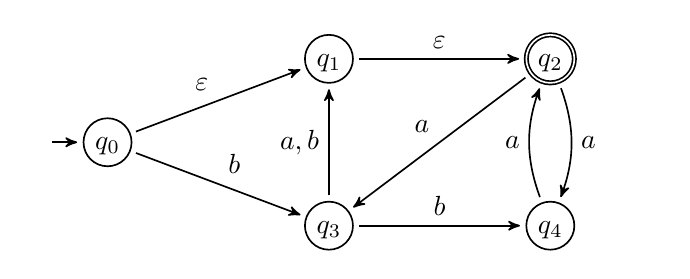
\begin{tikzpicture}[%
            ->,
            >=stealth',
            semithick,
            initial text=,
            shorten <=2pt,   
            shorten >=2pt,
            auto, 
            on grid,
            node distance=7ex and 8em,
            every state/.style={minimum size=0pt,inner sep=2pt,text height=1.5ex,text depth=.25ex},
            bend angle=20]
    \node[state,initial] (q_0) {$q_0$};
    \node[state] (q_1) [above right=of q_0] {$q_1$};
    \node[state,accepting] (q_2) [right=of q_1] {$q_2$};
    \node[state] (q_3) [below right=of q_0] {$q_3$};
    \node[state] (q_4) [right=of q_3] {$q_4$};
    \path[->]
    (q_0) edge node {$\varepsilon$} (q_1)
    (q_0) edge node {$b$} (q_3)
    (q_3) edge node {$a, b$} (q_1)
    (q_1) edge node {$\varepsilon$} (q_2)
    (q_2) edge node[above left] {$a$} (q_3)
    (q_2) edge[bend left] node {$a$} (q_4)
    (q_3) edge node {$b$} (q_4)
    (q_4) edge [bend left] node {$a$} (q_2) 
    (q_4) edge [loop right, white] node [white] {$a,b$} (q_4) ;
\end{tikzpicture}


\begin{exercise}
Gegeben ist der regul\"are Ausdruck $\alpha = (bb)^*a$.
  \begin{enumerate}
    \item Geben Sie f\"ur $\alpha$ die {\it{Nerode}}-Rechtskongruenz $\;\simeq_{L(\alpha)}\;$ an.
    \item Geben Sie einen minimalen DFA ${\mathcal M}$ an mit $L({\mathcal M})= L(\alpha)$.
  \end{enumerate} 
\end{exercise}


\newcommand{\simquot}[1]{#1/_{\!\!{\sim}}}

\begin{exercise}
  Beweisen Sie Lemma~$\varheartsuit$ aus Vorlesung~8:

  \begin{center}
    Sei $\mathcal{M} = \tuple{Q, \Sigma, \delta, q_{0}, F}$ ein totaler DFA und
    $\simquot{\mathcal{M}} = \tuple{\simquot{Q}, \Sigma, \delta_{\sim},
      [q_{0}]_{\sim}, \simquot{F}}$ der zugehörige Quotientenautomat. Dann gilt für beliebige $q \in Q$ und
    $w \in \Sigma^{*}$:
    \begin{equation*}
      [\delta(q, w)]_{\sim} = \delta_{\sim}([q]_{\sim}, w).
    \end{equation*}
  \end{center}

  Hinweis: Induktion über $|w|$.
\end{exercise}


\end{document}

%%% Local Variables:
%%% mode: latex
%%% TeX-master: t
%%% End:
